\documentclass[1p]{elsarticle_modified}
%\bibliographystyle{elsarticle-num}

%\usepackage[colorlinks]{hyperref}
%\usepackage{abbrmath_seonhwa} %\Abb, \Ascr, \Acal ,\Abf, \Afrak
\usepackage{amsfonts}
\usepackage{amssymb}
\usepackage{amsmath}
\usepackage{amsthm}
\usepackage{scalefnt}
\usepackage{amsbsy}
\usepackage{kotex}
\usepackage{caption}
\usepackage{subfig}
\usepackage{color}
\usepackage{graphicx}
\usepackage{xcolor} %% white, black, red, green, blue, cyan, magenta, yellow
\usepackage{float}
\usepackage{setspace}
\usepackage{hyperref}

\usepackage{tikz}
\usetikzlibrary{arrows}

\usepackage{multirow}
\usepackage{array} % fixed length table
\usepackage{hhline}

%%%%%%%%%%%%%%%%%%%%%
\makeatletter
\renewcommand*\env@matrix[1][\arraystretch]{%
	\edef\arraystretch{#1}%
	\hskip -\arraycolsep
	\let\@ifnextchar\new@ifnextchar
	\array{*\c@MaxMatrixCols c}}
\makeatother %https://tex.stackexchange.com/questions/14071/how-can-i-increase-the-line-spacing-in-a-matrix
%%%%%%%%%%%%%%%

\usepackage[normalem]{ulem}

\newcommand{\msout}[1]{\ifmmode\text{\sout{\ensuremath{#1}}}\else\sout{#1}\fi}
%SOURCE: \msout is \stkout macro in https://tex.stackexchange.com/questions/20609/strikeout-in-math-mode

\newcommand{\cancel}[1]{
	\ifmmode
	{\color{red}\msout{#1}}
	\else
	{\color{red}\sout{#1}}
	\fi
}

\newcommand{\add}[1]{
	{\color{blue}\uwave{#1}}
}

\newcommand{\replace}[2]{
	\ifmmode
	{\color{red}\msout{#1}}{\color{blue}\uwave{#2}}
	\else
	{\color{red}\sout{#1}}{\color{blue}\uwave{#2}}
	\fi
}

\newcommand{\Sol}{\mathcal{S}} %segment
\newcommand{\D}{D} %diagram
\newcommand{\A}{\mathcal{A}} %arc


%%%%%%%%%%%%%%%%%%%%%%%%%%%%%5 test

\def\sl{\operatorname{\textup{SL}}(2,\Cbb)}
\def\psl{\operatorname{\textup{PSL}}(2,\Cbb)}
\def\quan{\mkern 1mu \triangleright \mkern 1mu}

\theoremstyle{definition}
\newtheorem{thm}{Theorem}[section]
\newtheorem{prop}[thm]{Proposition}
\newtheorem{lem}[thm]{Lemma}
\newtheorem{ques}[thm]{Question}
\newtheorem{cor}[thm]{Corollary}
\newtheorem{defn}[thm]{Definition}
\newtheorem{exam}[thm]{Example}
\newtheorem{rmk}[thm]{Remark}
\newtheorem{alg}[thm]{Algorithm}

\newcommand{\I}{\sqrt{-1}}
\begin{document}

%\begin{frontmatter}
%
%\title{Boundary parabolic representations of knots up to 8 crossings}
%
%%% Group authors per affiliation:
%\author{Yunhi Cho} 
%\address{Department of Mathematics, University of Seoul, Seoul, Korea}
%\ead{yhcho@uos.ac.kr}
%
%
%\author{Seonhwa Kim} %\fnref{s_kim}}
%\address{Center for Geometry and Physics, Institute for Basic Science, Pohang, 37673, Korea}
%\ead{ryeona17@ibs.re.kr}
%
%\author{Hyuk Kim}
%\address{Department of Mathematical Sciences, Seoul National University, Seoul 08826, Korea}
%\ead{hyukkim@snu.ac.kr}
%
%\author{Seokbeom Yoon}
%\address{Department of Mathematical Sciences, Seoul National University, Seoul, 08826,  Korea}
%\ead{sbyoon15@snu.ac.kr}
%
%\begin{abstract}
%We find all boundary parabolic representation of knots up to 8 crossings.
%
%\end{abstract}
%\begin{keyword}
%    \MSC[2010] 57M25 
%\end{keyword}
%
%\end{frontmatter}

%\linenumbers
%\tableofcontents
%
\newcommand\colored[1]{\textcolor{white}{\rule[-0.35ex]{0.8em}{1.4ex}}\kern-0.8em\color{red} #1}%
%\newcommand\colored[1]{\textcolor{white}{ #1}\kern-2.17ex	\textcolor{white}{ #1}\kern-1.81ex	\textcolor{white}{ #1}\kern-2.15ex\color{red}#1	}

{\Large $\underline{12n_{0313}~(K12n_{0313})}$}

\setlength{\tabcolsep}{10pt}
\renewcommand{\arraystretch}{1.6}
\vspace{1cm}\begin{tabular}{m{100pt}>{\centering\arraybackslash}m{274pt}}
\multirow{5}{120pt}{
	\centering
	\includegraphics[width=112pt]{../../../GIT/diagram.site/Diagrams/png/2402_12n_0313.png}\\
\ \ \ A knot diagram\footnotemark}&
\allowdisplaybreaks
\textbf{Linearized knot diagam} \\
\cline{2-2}
 &
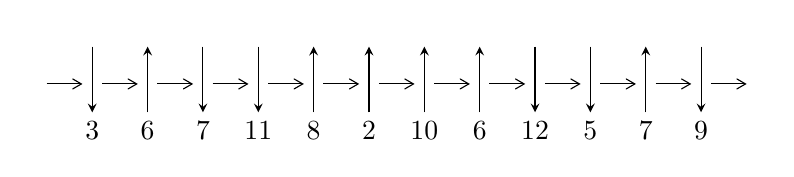
\begin{tikzpicture}[x=20pt, y=17pt]
	% nodes
	\node (C0) at (0, 0) {};
	\node (C1) at (1, 0) {};
	\node (C1U) at (1, +1) {};
	\node (C1D) at (1, -1) {3};

	\node (C2) at (2, 0) {};
	\node (C2U) at (2, +1) {};
	\node (C2D) at (2, -1) {6};

	\node (C3) at (3, 0) {};
	\node (C3U) at (3, +1) {};
	\node (C3D) at (3, -1) {7};

	\node (C4) at (4, 0) {};
	\node (C4U) at (4, +1) {};
	\node (C4D) at (4, -1) {11};

	\node (C5) at (5, 0) {};
	\node (C5U) at (5, +1) {};
	\node (C5D) at (5, -1) {8};

	\node (C6) at (6, 0) {};
	\node (C6U) at (6, +1) {};
	\node (C6D) at (6, -1) {2};

	\node (C7) at (7, 0) {};
	\node (C7U) at (7, +1) {};
	\node (C7D) at (7, -1) {10};

	\node (C8) at (8, 0) {};
	\node (C8U) at (8, +1) {};
	\node (C8D) at (8, -1) {6};

	\node (C9) at (9, 0) {};
	\node (C9U) at (9, +1) {};
	\node (C9D) at (9, -1) {12};

	\node (C10) at (10, 0) {};
	\node (C10U) at (10, +1) {};
	\node (C10D) at (10, -1) {5};

	\node (C11) at (11, 0) {};
	\node (C11U) at (11, +1) {};
	\node (C11D) at (11, -1) {7};

	\node (C12) at (12, 0) {};
	\node (C12U) at (12, +1) {};
	\node (C12D) at (12, -1) {9};
	\node (C13) at (13, 0) {};

	% arrows
	\draw[->,>={angle 60}]
	(C0) edge (C1) (C1) edge (C2) (C2) edge (C3) (C3) edge (C4) (C4) edge (C5) (C5) edge (C6) (C6) edge (C7) (C7) edge (C8) (C8) edge (C9) (C9) edge (C10) (C10) edge (C11) (C11) edge (C12) (C12) edge (C13) ;	\draw[->,>=stealth]
	(C1U) edge (C1D) (C2D) edge (C2U) (C3U) edge (C3D) (C4U) edge (C4D) (C5D) edge (C5U) (C6D) edge (C6U) (C7D) edge (C7U) (C8D) edge (C8U) (C9U) edge (C9D) (C10U) edge (C10D) (C11D) edge (C11U) (C12U) edge (C12D) ;
	\end{tikzpicture} \\
\hhline{~~} \\& 
\textbf{Solving Sequence} \\ \cline{2-2} 
 &
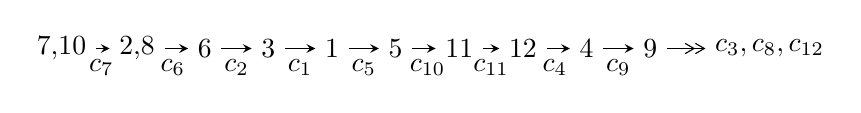
\begin{tikzpicture}[x=23pt, y=7pt]
	% node
	\node (A0) at (-1/8, 0) {7,10};
	\node (A1) at (17/16, 0) {2,8};
	\node (A2) at (17/8, 0) {6};
	\node (A3) at (25/8, 0) {3};
	\node (A4) at (33/8, 0) {1};
	\node (A5) at (41/8, 0) {5};
	\node (A6) at (49/8, 0) {11};
	\node (A7) at (57/8, 0) {12};
	\node (A8) at (65/8, 0) {4};
	\node (A9) at (73/8, 0) {9};
	\node (C1) at (1/2, -1) {$c_{7}$};
	\node (C2) at (13/8, -1) {$c_{6}$};
	\node (C3) at (21/8, -1) {$c_{2}$};
	\node (C4) at (29/8, -1) {$c_{1}$};
	\node (C5) at (37/8, -1) {$c_{5}$};
	\node (C6) at (45/8, -1) {$c_{10}$};
	\node (C7) at (53/8, -1) {$c_{11}$};
	\node (C8) at (61/8, -1) {$c_{4}$};
	\node (C9) at (69/8, -1) {$c_{9}$};
	\node (A10) at (11, 0) {$c_{3},c_{8},c_{12}$};

	% edge
	\draw[->,>=stealth]	
	(A0) edge (A1) (A1) edge (A2) (A2) edge (A3) (A3) edge (A4) (A4) edge (A5) (A5) edge (A6) (A6) edge (A7) (A7) edge (A8) (A8) edge (A9) ;
	\draw[->>,>={angle 60}]	
	(A9) edge (A10);
\end{tikzpicture} \\ 

\end{tabular} \\

\footnotetext{
The image of knot diagram is generated by the software ``\textbf{Draw programme}" developed by Andrew Bartholomew(\url{http://www.layer8.co.uk/maths/draw/index.htm\#Running-draw}), where we modified some parts for our purpose(\url{https://github.com/CATsTAILs/LinksPainter}).
}\phantom \\ \newline 
\centering \textbf{Ideals for irreducible components\footnotemark of $X_{\text{par}}$} 
 
\begin{align*}
I^u_{1}&=\langle 
-41545 u^{14}+62711 u^{13}+\cdots+83381 b+22577,\\
\phantom{I^u_{1}}&\phantom{= \langle  }-56191 u^{14}+116417 u^{13}+\cdots+83381 a+99262,\\
\phantom{I^u_{1}}&\phantom{= \langle  }u^{15}-2 u^{14}+u^{13}+2 u^{12}+4 u^{11}-12 u^{10}+7 u^9+4 u^8+10 u^7-28 u^6+13 u^5+3 u^4-5 u^3+5 u^2-3 u+1\rangle \\
I^u_{2}&=\langle 
-2 u^8-6 u^7-7 u^6+4 u^5+15 u^4+8 u^3-10 u^2+b-15 u-5,\\
\phantom{I^u_{2}}&\phantom{= \langle  }-2 u^8-6 u^7-8 u^6+3 u^5+15 u^4+12 u^3-9 u^2+a-16 u-8,\\
\phantom{I^u_{2}}&\phantom{= \langle  }u^9+3 u^8+4 u^7- u^6-7 u^5-6 u^4+3 u^3+8 u^2+5 u+1\rangle \\
I^u_{3}&=\langle 
- u^5-3 u^4-3 u^3- u^2+b- u-1,\;- u^5-3 u^4-3 u^3- u^2+a- u-1,\;u^6+3 u^5+4 u^4+3 u^3+3 u^2+2 u+1\rangle \\
\\
\end{align*}
\raggedright * 3 irreducible components of $\dim_{\mathbb{C}}=0$, with total 30 representations.\\
\footnotetext{All coefficients of polynomials are rational numbers. But the coefficients are sometimes approximated in decimal forms when there is not enough margin.}
\newpage
\renewcommand{\arraystretch}{1}
\centering \section*{I. $I^u_{1}= \langle -41545 u^{14}+62711 u^{13}+\cdots+83381 b+22577,\;-5.62\times10^{4} u^{14}+1.16\times10^{5} u^{13}+\cdots+8.34\times10^{4} a+9.93\times10^{4},\;u^{15}-2 u^{14}+\cdots-3 u+1 \rangle$}
\flushleft \textbf{(i) Arc colorings}\\
\begin{tabular}{m{7pt} m{180pt} m{7pt} m{180pt} }
\flushright $a_{7}=$&$\begin{pmatrix}1\\0\end{pmatrix}$ \\
\flushright $a_{10}=$&$\begin{pmatrix}0\\u\end{pmatrix}$ \\
\flushright $a_{2}=$&$\begin{pmatrix}0.673907 u^{14}-1.39621 u^{13}+\cdots+1.05994 u-1.19046\\0.498255 u^{14}-0.752102 u^{13}+\cdots+1.28760 u-0.270769\end{pmatrix}$ \\
\flushright $a_{8}=$&$\begin{pmatrix}1\\- u^2\end{pmatrix}$ \\
\flushright $a_{6}=$&$\begin{pmatrix}-0.828462 u^{14}+1.02276 u^{13}+\cdots-3.35724 u+0.995263\\0.862870 u^{14}-1.23046 u^{13}+\cdots+2.60733 u-1.50841\end{pmatrix}$ \\
\flushright $a_{3}=$&$\begin{pmatrix}0.651875 u^{14}-1.12205 u^{13}+\cdots+0.0277281 u-0.890826\\0.0258572 u^{14}-0.477447 u^{13}+\cdots+0.528826 u-0.465442\end{pmatrix}$ \\
\flushright $a_{1}=$&$\begin{pmatrix}0.0135522 u^{14}-0.409794 u^{13}+\cdots-1.03081 u-0.189216\\-0.240930 u^{14}+0.319773 u^{13}+\cdots-1.40889 u+0.529341\end{pmatrix}$ \\
\flushright $a_{5}=$&$\begin{pmatrix}-1.22448 u^{14}+1.65231 u^{13}+\cdots-4.89055 u+1.86951\\1.00210 u^{14}-1.42187 u^{13}+\cdots+2.69877 u-1.67090\end{pmatrix}$ \\
\flushright $a_{11}=$&$\begin{pmatrix}-0.582255 u^{14}+0.870858 u^{13}+\cdots-0.677157 u+1.06481\\0.560224 u^{14}-0.596707 u^{13}+\cdots+1.64494 u-0.765174\end{pmatrix}$ \\
\flushright $a_{12}=$&$\begin{pmatrix}-0.0220314 u^{14}+0.274151 u^{13}+\cdots+0.967786 u+0.299637\\0.560224 u^{14}-0.596707 u^{13}+\cdots+1.64494 u-0.765174\end{pmatrix}$ \\
\flushright $a_{4}=$&$\begin{pmatrix}0.626018 u^{14}-0.644607 u^{13}+\cdots-0.501097 u-0.425385\\0.0258572 u^{14}-0.477447 u^{13}+\cdots+0.528826 u-0.465442\end{pmatrix}$ \\
\flushright $a_{9}=$&$\begin{pmatrix}0.539284 u^{14}-0.621928 u^{13}+\cdots+1.09609 u-0.0144038\\-0.201365 u^{14}+0.389765 u^{13}+\cdots+0.0153152 u+0.510560\end{pmatrix}$\\&\end{tabular}
\flushleft \textbf{(ii) Obstruction class $= -1$}\\~\\
\flushleft \textbf{(iii) Cusp Shapes $= -\frac{473234}{83381} u^{14}+\frac{693041}{83381} u^{13}+\cdots-\frac{1183972}{83381} u+\frac{479281}{83381}$}\\~\\
\newpage\renewcommand{\arraystretch}{1}
\flushleft \textbf{(iv) u-Polynomials at the component}\newline \\
\begin{tabular}{m{50pt}|m{274pt}}
Crossings & \hspace{64pt}u-Polynomials at each crossing \\
\hline $$\begin{aligned}c_{1}\end{aligned}$$&$\begin{aligned}
&u^{15}+19 u^{14}+\cdots-13464 u-2209
\end{aligned}$\\
\hline $$\begin{aligned}c_{2},c_{6}\end{aligned}$$&$\begin{aligned}
&u^{15}- u^{14}+\cdots+52 u-47
\end{aligned}$\\
\hline $$\begin{aligned}c_{3}\end{aligned}$$&$\begin{aligned}
&u^{15}+16 u^{14}+\cdots+571220 u-516295
\end{aligned}$\\
\hline $$\begin{aligned}c_{4},c_{10}\end{aligned}$$&$\begin{aligned}
&u^{15}-4 u^{14}+\cdots+124 u-11
\end{aligned}$\\
\hline $$\begin{aligned}c_{5},c_{8}\end{aligned}$$&$\begin{aligned}
&u^{15}+2 u^{14}+\cdots-193 u-131
\end{aligned}$\\
\hline $$\begin{aligned}c_{7}\end{aligned}$$&$\begin{aligned}
&u^{15}+2 u^{14}+\cdots-3 u-1
\end{aligned}$\\
\hline $$\begin{aligned}c_{9},c_{12}\end{aligned}$$&$\begin{aligned}
&u^{15}-4 u^{13}+\cdots+95 u-23
\end{aligned}$\\
\hline $$\begin{aligned}c_{11}\end{aligned}$$&$\begin{aligned}
&u^{15}-10 u^{14}+\cdots+1544 u-1961
\end{aligned}$\\
\hline
\end{tabular}\\~\\
\newpage\renewcommand{\arraystretch}{1}
\flushleft \textbf{(v) Riley Polynomials at the component}\newline \\
\begin{tabular}{m{50pt}|m{274pt}}
Crossings & \hspace{64pt}Riley Polynomials at each crossing \\
\hline $$\begin{aligned}c_{1}\end{aligned}$$&$\begin{aligned}
&y^{15}+27 y^{14}+\cdots+93308080 y-4879681
\end{aligned}$\\
\hline $$\begin{aligned}c_{2},c_{6}\end{aligned}$$&$\begin{aligned}
&y^{15}+19 y^{14}+\cdots-13464 y-2209
\end{aligned}$\\
\hline $$\begin{aligned}c_{3}\end{aligned}$$&$\begin{aligned}
&y^{15}-268 y^{14}+\cdots-3653087564750 y-266560527025
\end{aligned}$\\
\hline $$\begin{aligned}c_{4},c_{10}\end{aligned}$$&$\begin{aligned}
&y^{15}+28 y^{14}+\cdots+22856 y-121
\end{aligned}$\\
\hline $$\begin{aligned}c_{5},c_{8}\end{aligned}$$&$\begin{aligned}
&y^{15}-26 y^{14}+\cdots+40393 y-17161
\end{aligned}$\\
\hline $$\begin{aligned}c_{7}\end{aligned}$$&$\begin{aligned}
&y^{15}-2 y^{14}+\cdots- y-1
\end{aligned}$\\
\hline $$\begin{aligned}c_{9},c_{12}\end{aligned}$$&$\begin{aligned}
&y^{15}-8 y^{14}+\cdots+2493 y-529
\end{aligned}$\\
\hline $$\begin{aligned}c_{11}\end{aligned}$$&$\begin{aligned}
&y^{15}+12 y^{14}+\cdots-79903546 y-3845521
\end{aligned}$\\
\hline
\end{tabular}\\~\\
\newpage\flushleft \textbf{(vi) Complex Volumes and Cusp Shapes}
$$\begin{array}{c|c|c}  
\text{Solutions to }I^u_{1}& \I (\text{vol} + \sqrt{-1}CS) & \text{Cusp shape}\\
 \hline 
\begin{aligned}
u &= \phantom{-}0.898089 + 0.122561 I \\
a &= \phantom{-}0.851665 + 0.429887 I \\
b &= -0.813523 - 0.857386 I\end{aligned}
 & \phantom{-}8.21514 + 3.43846 I & \phantom{-}8.39038 - 0.14759 I \\ \hline\begin{aligned}
u &= \phantom{-}0.898089 - 0.122561 I \\
a &= \phantom{-}0.851665 - 0.429887 I \\
b &= -0.813523 + 0.857386 I\end{aligned}
 & \phantom{-}8.21514 - 3.43846 I & \phantom{-}8.39038 + 0.14759 I \\ \hline\begin{aligned}
u &= -0.727637\phantom{ +0.000000I} \\
a &= \phantom{-}0.282926\phantom{ +0.000000I} \\
b &= \phantom{-}0.679431\phantom{ +0.000000I}\end{aligned}
 & \phantom{-}1.43379\phantom{ +0.000000I} & \phantom{-}8.32270\phantom{ +0.000000I} \\ \hline\begin{aligned}
u &= -0.776726 + 1.064100 I \\
a &= \phantom{-}0.198165 + 1.273550 I \\
b &= -0.90296 + 1.50976 I\end{aligned}
 & \phantom{-}1.61435 - 4.09120 I & \phantom{-}1.62171 + 2.87173 I \\ \hline\begin{aligned}
u &= -0.776726 - 1.064100 I \\
a &= \phantom{-}0.198165 - 1.273550 I \\
b &= -0.90296 - 1.50976 I\end{aligned}
 & \phantom{-}1.61435 + 4.09120 I & \phantom{-}1.62171 - 2.87173 I \\ \hline\begin{aligned}
u &= -1.20953 + 0.78183 I \\
a &= -0.907869 - 0.069228 I \\
b &= -0.45282 - 1.51307 I\end{aligned}
 & \phantom{-}3.12702 - 2.88040 I & \phantom{-}2.11466 + 1.70139 I \\ \hline\begin{aligned}
u &= -1.20953 - 0.78183 I \\
a &= -0.907869 + 0.069228 I \\
b &= -0.45282 + 1.51307 I\end{aligned}
 & \phantom{-}3.12702 + 2.88040 I & \phantom{-}2.11466 - 1.70139 I \\ \hline\begin{aligned}
u &= -0.067561 + 0.552036 I \\
a &= \phantom{-}1.49637 - 1.52360 I \\
b &= -0.032891 - 0.581799 I\end{aligned}
 & -1.07742 - 1.06518 I & -5.69949 + 4.71826 I \\ \hline\begin{aligned}
u &= -0.067561 - 0.552036 I \\
a &= \phantom{-}1.49637 + 1.52360 I \\
b &= -0.032891 + 0.581799 I\end{aligned}
 & -1.07742 + 1.06518 I & -5.69949 - 4.71826 I \\ \hline\begin{aligned}
u &= \phantom{-}0.402433 + 0.347088 I \\
a &= -1.35119 + 0.98940 I \\
b &= \phantom{-}0.547092 + 0.828723 I\end{aligned}
 & \phantom{-}0.07543 + 2.01877 I & \phantom{-}0.10830 - 4.30124 I\\
 \hline 
 \end{array}$$\newpage$$\begin{array}{c|c|c}  
\text{Solutions to }I^u_{1}& \I (\text{vol} + \sqrt{-1}CS) & \text{Cusp shape}\\
 \hline 
\begin{aligned}
u &= \phantom{-}0.402433 - 0.347088 I \\
a &= -1.35119 - 0.98940 I \\
b &= \phantom{-}0.547092 - 0.828723 I\end{aligned}
 & \phantom{-}0.07543 - 2.01877 I & \phantom{-}0.10830 + 4.30124 I \\ \hline\begin{aligned}
u &= \phantom{-}1.10914 + 1.03230 I \\
a &= -0.75781 + 1.35948 I \\
b &= \phantom{-}1.04371 + 1.80853 I\end{aligned}
 & -11.8911 + 11.0679 I & \phantom{-}2.10881 - 4.27183 I \\ \hline\begin{aligned}
u &= \phantom{-}1.10914 - 1.03230 I \\
a &= -0.75781 - 1.35948 I \\
b &= \phantom{-}1.04371 - 1.80853 I\end{aligned}
 & -11.8911 - 11.0679 I & \phantom{-}2.10881 + 4.27183 I \\ \hline\begin{aligned}
u &= \phantom{-}1.00798 + 1.14054 I \\
a &= \phantom{-}0.829204 - 0.703970 I \\
b &= \phantom{-}0.77167 - 1.94892 I\end{aligned}
 & -12.29490 - 3.15413 I & \phantom{-}1.69429 + 0.52217 I \\ \hline\begin{aligned}
u &= \phantom{-}1.00798 - 1.14054 I \\
a &= \phantom{-}0.829204 + 0.703970 I \\
b &= \phantom{-}0.77167 + 1.94892 I\end{aligned}
 & -12.29490 + 3.15413 I & \phantom{-}1.69429 - 0.52217 I\\
 \hline 
 \end{array}$$\newpage\newpage\renewcommand{\arraystretch}{1}
\centering \section*{II. $I^u_{2}= \langle -2 u^8-6 u^7+\cdots+b-5,\;-2 u^8-6 u^7+\cdots+a-8,\;u^9+3 u^8+\cdots+5 u+1 \rangle$}
\flushleft \textbf{(i) Arc colorings}\\
\begin{tabular}{m{7pt} m{180pt} m{7pt} m{180pt} }
\flushright $a_{7}=$&$\begin{pmatrix}1\\0\end{pmatrix}$ \\
\flushright $a_{10}=$&$\begin{pmatrix}0\\u\end{pmatrix}$ \\
\flushright $a_{2}=$&$\begin{pmatrix}2 u^8+6 u^7+8 u^6-3 u^5-15 u^4-12 u^3+9 u^2+16 u+8\\2 u^8+6 u^7+7 u^6-4 u^5-15 u^4-8 u^3+10 u^2+15 u+5\end{pmatrix}$ \\
\flushright $a_{8}=$&$\begin{pmatrix}1\\- u^2\end{pmatrix}$ \\
\flushright $a_{6}=$&$\begin{pmatrix}4 u^8+11 u^7+13 u^6-8 u^5-27 u^4-17 u^3+18 u^2+29 u+12\\u^8+2 u^7+2 u^6-3 u^5-4 u^4-2 u^3+5 u^2+3 u+1\end{pmatrix}$ \\
\flushright $a_{3}=$&$\begin{pmatrix}7 u^8+18 u^7+21 u^6-15 u^5-42 u^4-26 u^3+31 u^2+43 u+18\\2 u^7+4 u^6+3 u^5-7 u^4-8 u^3+10 u+5\end{pmatrix}$ \\
\flushright $a_{1}=$&$\begin{pmatrix}10 u^8+25 u^7+28 u^6-23 u^5-58 u^4-33 u^3+44 u^2+58 u+23\\-3 u^8-6 u^7-5 u^6+10 u^5+13 u^4+2 u^3-15 u^2-10 u\end{pmatrix}$ \\
\flushright $a_{5}=$&$\begin{pmatrix}3 u^8+9 u^7+11 u^6-5 u^5-23 u^4-15 u^3+13 u^2+25 u+10\\2 u^8+4 u^7+4 u^6-6 u^5-8 u^4-3 u^3+10 u^2+7 u+2\end{pmatrix}$ \\
\flushright $a_{11}=$&$\begin{pmatrix}9 u^8+22 u^7+23 u^6-23 u^5-51 u^4-23 u^3+42 u^2+49 u+15\\-4 u^8-10 u^7-10 u^6+11 u^5+24 u^4+9 u^3-20 u^2-22 u-5\end{pmatrix}$ \\
\flushright $a_{12}=$&$\begin{pmatrix}5 u^8+12 u^7+13 u^6-12 u^5-27 u^4-14 u^3+22 u^2+27 u+10\\-4 u^8-10 u^7-10 u^6+11 u^5+24 u^4+9 u^3-20 u^2-22 u-5\end{pmatrix}$ \\
\flushright $a_{4}=$&$\begin{pmatrix}7 u^8+16 u^7+17 u^6-18 u^5-35 u^4-18 u^3+31 u^2+33 u+13\\2 u^7+4 u^6+3 u^5-7 u^4-8 u^3+10 u+5\end{pmatrix}$ \\
\flushright $a_{9}=$&$\begin{pmatrix}-4 u^8-11 u^7-13 u^6+8 u^5+27 u^4+17 u^3-18 u^2-29 u-12\\-4 u^8-9 u^7-9 u^6+11 u^5+20 u^4+8 u^3-19 u^2-18 u-5\end{pmatrix}$\\&\end{tabular}
\flushleft \textbf{(ii) Obstruction class $= 1$}\\~\\
\flushleft \textbf{(iii) Cusp Shapes $= -6 u^8-13 u^7-11 u^6+19 u^5+27 u^4+5 u^3-30 u^2-16 u-2$}\\~\\
\newpage\renewcommand{\arraystretch}{1}
\flushleft \textbf{(iv) u-Polynomials at the component}\newline \\
\begin{tabular}{m{50pt}|m{274pt}}
Crossings & \hspace{64pt}u-Polynomials at each crossing \\
\hline $$\begin{aligned}c_{1}\end{aligned}$$&$\begin{aligned}
&u^9-3 u^8+6 u^7-9 u^6+12 u^5-10 u^4+3 u^3+4 u^2-4 u+1
\end{aligned}$\\
\hline $$\begin{aligned}c_{2}\end{aligned}$$&$\begin{aligned}
&u^9- u^8+2 u^7- u^6+2 u^5+u^3+2 u^2+1
\end{aligned}$\\
\hline $$\begin{aligned}c_{3}\end{aligned}$$&$\begin{aligned}
&u^9+u^8+5 u^7+10 u^6+u^5+u^4+12 u^3+9 u^2+2 u+1
\end{aligned}$\\
\hline $$\begin{aligned}c_{4}\end{aligned}$$&$\begin{aligned}
&u^9+5 u^7+u^6+7 u^5+5 u^4+u^3+6 u^2-2 u+1
\end{aligned}$\\
\hline $$\begin{aligned}c_{5}\end{aligned}$$&$\begin{aligned}
&u^9+3 u^8+u^7-5 u^6-5 u^5+4 u^4+9 u^3-4 u+1
\end{aligned}$\\
\hline $$\begin{aligned}c_{6}\end{aligned}$$&$\begin{aligned}
&u^9+u^8+2 u^7+u^6+2 u^5+u^3-2 u^2-1
\end{aligned}$\\
\hline $$\begin{aligned}c_{7}\end{aligned}$$&$\begin{aligned}
&u^9+3 u^8+4 u^7- u^6-7 u^5-6 u^4+3 u^3+8 u^2+5 u+1
\end{aligned}$\\
\hline $$\begin{aligned}c_{8}\end{aligned}$$&$\begin{aligned}
&u^9-3 u^8+u^7+5 u^6-5 u^5-4 u^4+9 u^3-4 u-1
\end{aligned}$\\
\hline $$\begin{aligned}c_{9}\end{aligned}$$&$\begin{aligned}
&u^9+2 u^7- u^6-2 u^4- u^3-2 u^2- u-1
\end{aligned}$\\
\hline $$\begin{aligned}c_{10}\end{aligned}$$&$\begin{aligned}
&u^9+5 u^7- u^6+7 u^5-5 u^4+u^3-6 u^2-2 u-1
\end{aligned}$\\
\hline $$\begin{aligned}c_{11}\end{aligned}$$&$\begin{aligned}
&u^9+6 u^8+10 u^7+4 u^6+11 u^5+23 u^4+10 u^3+6 u^2+13 u+5
\end{aligned}$\\
\hline $$\begin{aligned}c_{12}\end{aligned}$$&$\begin{aligned}
&u^9+2 u^7+u^6+2 u^4- u^3+2 u^2- u+1
\end{aligned}$\\
\hline
\end{tabular}\\~\\
\newpage\renewcommand{\arraystretch}{1}
\flushleft \textbf{(v) Riley Polynomials at the component}\newline \\
\begin{tabular}{m{50pt}|m{274pt}}
Crossings & \hspace{64pt}Riley Polynomials at each crossing \\
\hline $$\begin{aligned}c_{1}\end{aligned}$$&$\begin{aligned}
&y^9+3 y^8+6 y^7+9 y^6+16 y^5+2 y^4+11 y^3-20 y^2+8 y-1
\end{aligned}$\\
\hline $$\begin{aligned}c_{2},c_{6}\end{aligned}$$&$\begin{aligned}
&y^9+3 y^8+6 y^7+9 y^6+12 y^5+10 y^4+3 y^3-4 y^2-4 y-1
\end{aligned}$\\
\hline $$\begin{aligned}c_{3}\end{aligned}$$&$\begin{aligned}
&y^9+9 y^8+7 y^7-68 y^6+87 y^5-139 y^4+110 y^3-35 y^2-14 y-1
\end{aligned}$\\
\hline $$\begin{aligned}c_{4},c_{10}\end{aligned}$$&$\begin{aligned}
&y^9+10 y^8+39 y^7+71 y^6+45 y^5-43 y^4-89 y^3-50 y^2-8 y-1
\end{aligned}$\\
\hline $$\begin{aligned}c_{5},c_{8}\end{aligned}$$&$\begin{aligned}
&y^9-7 y^8+21 y^7-41 y^6+75 y^5-120 y^4+131 y^3-80 y^2+16 y-1
\end{aligned}$\\
\hline $$\begin{aligned}c_{7}\end{aligned}$$&$\begin{aligned}
&y^9- y^8+8 y^7-15 y^6+23 y^5-28 y^4+37 y^3-22 y^2+9 y-1
\end{aligned}$\\
\hline $$\begin{aligned}c_{9},c_{12}\end{aligned}$$&$\begin{aligned}
&y^9+4 y^8+4 y^7-3 y^6-10 y^5-12 y^4-9 y^3-6 y^2-3 y-1
\end{aligned}$\\
\hline $$\begin{aligned}c_{11}\end{aligned}$$&$\begin{aligned}
&y^9-16 y^8+74 y^7-52 y^6+91 y^5-157 y^4+70 y^3-6 y^2+109 y-25
\end{aligned}$\\
\hline
\end{tabular}\\~\\
\newpage\flushleft \textbf{(vi) Complex Volumes and Cusp Shapes}
$$\begin{array}{c|c|c}  
\text{Solutions to }I^u_{2}& \I (\text{vol} + \sqrt{-1}CS) & \text{Cusp shape}\\
 \hline 
\begin{aligned}
u &= \phantom{-}1.072880 + 0.352289 I \\
a &= -1.056530 - 0.568290 I \\
b &= -0.054519 + 0.730817 I\end{aligned}
 & \phantom{-}7.45475 + 1.27338 I & \phantom{-}5.64490 - 0.43727 I \\ \hline\begin{aligned}
u &= \phantom{-}1.072880 - 0.352289 I \\
a &= -1.056530 + 0.568290 I \\
b &= -0.054519 - 0.730817 I\end{aligned}
 & \phantom{-}7.45475 - 1.27338 I & \phantom{-}5.64490 + 0.43727 I \\ \hline\begin{aligned}
u &= -0.692006 + 0.938897 I \\
a &= -0.73796 - 1.40715 I \\
b &= \phantom{-}0.497907 - 0.965644 I\end{aligned}
 & -0.18404 - 4.42541 I & -3.46550 + 5.77063 I \\ \hline\begin{aligned}
u &= -0.692006 - 0.938897 I \\
a &= -0.73796 + 1.40715 I \\
b &= \phantom{-}0.497907 + 0.965644 I\end{aligned}
 & -0.18404 + 4.42541 I & -3.46550 - 5.77063 I \\ \hline\begin{aligned}
u &= -0.654771 + 0.355732 I \\
a &= \phantom{-}1.208170 + 0.025665 I \\
b &= -0.976768 + 0.741048 I\end{aligned}
 & \phantom{-}7.61597 - 3.90243 I & \phantom{-}0.00196 + 5.82113 I \\ \hline\begin{aligned}
u &= -0.654771 - 0.355732 I \\
a &= \phantom{-}1.208170 - 0.025665 I \\
b &= -0.976768 - 0.741048 I\end{aligned}
 & \phantom{-}7.61597 + 3.90243 I & \phantom{-}0.00196 - 5.82113 I \\ \hline\begin{aligned}
u &= -0.396548\phantom{ +0.000000I} \\
a &= \phantom{-}3.50035\phantom{ +0.000000I} \\
b &= \phantom{-}0.810638\phantom{ +0.000000I}\end{aligned}
 & \phantom{-}0.137068\phantom{ +0.000000I} & -0.229590\phantom{ +0.000000I} \\ \hline\begin{aligned}
u &= -1.02783 + 1.24961 I \\
a &= \phantom{-}0.336146 + 1.247420 I \\
b &= -0.371939 + 1.075240 I\end{aligned}
 & \phantom{-}3.13906 - 5.52199 I & \phantom{-}4.93343 + 8.47719 I \\ \hline\begin{aligned}
u &= -1.02783 - 1.24961 I \\
a &= \phantom{-}0.336146 - 1.247420 I \\
b &= -0.371939 - 1.075240 I\end{aligned}
 & \phantom{-}3.13906 + 5.52199 I & \phantom{-}4.93343 - 8.47719 I\\
 \hline 
 \end{array}$$\newpage\newpage\renewcommand{\arraystretch}{1}
\centering \section*{III. $I^u_{3}= \langle - u^5-3 u^4-3 u^3- u^2+b- u-1,\;- u^5-3 u^4-3 u^3- u^2+a- u-1,\;u^6+3 u^5+4 u^4+3 u^3+3 u^2+2 u+1 \rangle$}
\flushleft \textbf{(i) Arc colorings}\\
\begin{tabular}{m{7pt} m{180pt} m{7pt} m{180pt} }
\flushright $a_{7}=$&$\begin{pmatrix}1\\0\end{pmatrix}$ \\
\flushright $a_{10}=$&$\begin{pmatrix}0\\u\end{pmatrix}$ \\
\flushright $a_{2}=$&$\begin{pmatrix}u^5+3 u^4+3 u^3+u^2+u+1\\u^5+3 u^4+3 u^3+u^2+u+1\end{pmatrix}$ \\
\flushright $a_{8}=$&$\begin{pmatrix}1\\- u^2\end{pmatrix}$ \\
\flushright $a_{6}=$&$\begin{pmatrix}u^5+3 u^4+4 u^3+3 u^2+3 u+2\\u^5+3 u^4+4 u^3+3 u^2+3 u+1\end{pmatrix}$ \\
\flushright $a_{3}=$&$\begin{pmatrix}2 u^5+5 u^4+4 u^3+u^2+3 u+2\\u^5+2 u^4+u^3+2 u+1\end{pmatrix}$ \\
\flushright $a_{1}=$&$\begin{pmatrix}u^5+2 u^4+2 u^3+2 u^2+3 u\\u^5+3 u^4+4 u^3+3 u^2+2 u\end{pmatrix}$ \\
\flushright $a_{5}=$&$\begin{pmatrix}u+1\\u^5+3 u^4+3 u^3+2 u^2+2 u+1\end{pmatrix}$ \\
\flushright $a_{11}=$&$\begin{pmatrix}- u^3-2 u^2- u\\u^5+2 u^4+2 u^3+2 u^2+3 u+1\end{pmatrix}$ \\
\flushright $a_{12}=$&$\begin{pmatrix}u^5+2 u^4+u^3+2 u+1\\u^5+2 u^4+2 u^3+2 u^2+3 u+1\end{pmatrix}$ \\
\flushright $a_{4}=$&$\begin{pmatrix}u^5+3 u^4+3 u^3+u^2+u+1\\u^5+2 u^4+u^3+2 u+1\end{pmatrix}$ \\
\flushright $a_{9}=$&$\begin{pmatrix}- u^5-2 u^4- u^3+u^2+1\\u^4+3 u^3+3 u^2+2 u+1\end{pmatrix}$\\&\end{tabular}
\flushleft \textbf{(ii) Obstruction class $= 1$}\\~\\
\flushleft \textbf{(iii) Cusp Shapes $= 2 u^5+2 u^4-2 u^2- u+1$}\\~\\
\newpage\renewcommand{\arraystretch}{1}
\flushleft \textbf{(iv) u-Polynomials at the component}\newline \\
\begin{tabular}{m{50pt}|m{274pt}}
Crossings & \hspace{64pt}u-Polynomials at each crossing \\
\hline $$\begin{aligned}c_{1}\end{aligned}$$&$\begin{aligned}
&u^6-4 u^5+8 u^4-9 u^3+8 u^2-4 u+1
\end{aligned}$\\
\hline $$\begin{aligned}c_{2},c_{12}\end{aligned}$$&$\begin{aligned}
&u^6+2 u^4+u^3+2 u^2+1
\end{aligned}$\\
\hline $$\begin{aligned}c_{3}\end{aligned}$$&$\begin{aligned}
&u^6+3 u^5+4 u^4+6 u^3+6 u^2+2 u+1
\end{aligned}$\\
\hline $$\begin{aligned}c_{4}\end{aligned}$$&$\begin{aligned}
&(u^3+u^2+2 u+1)^2
\end{aligned}$\\
\hline $$\begin{aligned}c_{5}\end{aligned}$$&$\begin{aligned}
&u^6- u^5-3 u^4+4 u^2+3 u+1
\end{aligned}$\\
\hline $$\begin{aligned}c_{6},c_{9}\end{aligned}$$&$\begin{aligned}
&u^6+2 u^4- u^3+2 u^2+1
\end{aligned}$\\
\hline $$\begin{aligned}c_{7}\end{aligned}$$&$\begin{aligned}
&u^6+3 u^5+4 u^4+3 u^3+3 u^2+2 u+1
\end{aligned}$\\
\hline $$\begin{aligned}c_{8}\end{aligned}$$&$\begin{aligned}
&u^6+u^5-3 u^4+4 u^2-3 u+1
\end{aligned}$\\
\hline $$\begin{aligned}c_{10}\end{aligned}$$&$\begin{aligned}
&(u^3- u^2+2 u-1)^2
\end{aligned}$\\
\hline $$\begin{aligned}c_{11}\end{aligned}$$&$\begin{aligned}
&u^6+2 u^5+4 u^4+6 u^3+4 u^2+5 u+5
\end{aligned}$\\
\hline
\end{tabular}\\~\\
\newpage\renewcommand{\arraystretch}{1}
\flushleft \textbf{(v) Riley Polynomials at the component}\newline \\
\begin{tabular}{m{50pt}|m{274pt}}
Crossings & \hspace{64pt}Riley Polynomials at each crossing \\
\hline $$\begin{aligned}c_{1}\end{aligned}$$&$\begin{aligned}
&y^6+8 y^4+17 y^3+8 y^2+1
\end{aligned}$\\
\hline $$\begin{aligned}c_{2},c_{6},c_{9}\\c_{12}\end{aligned}$$&$\begin{aligned}
&y^6+4 y^5+8 y^4+9 y^3+8 y^2+4 y+1
\end{aligned}$\\
\hline $$\begin{aligned}c_{3}\end{aligned}$$&$\begin{aligned}
&y^6- y^5-8 y^4+2 y^3+20 y^2+8 y+1
\end{aligned}$\\
\hline $$\begin{aligned}c_{4},c_{10}\end{aligned}$$&$\begin{aligned}
&(y^3+3 y^2+2 y-1)^2
\end{aligned}$\\
\hline $$\begin{aligned}c_{5},c_{8}\end{aligned}$$&$\begin{aligned}
&y^6-7 y^5+17 y^4-16 y^3+10 y^2- y+1
\end{aligned}$\\
\hline $$\begin{aligned}c_{7}\end{aligned}$$&$\begin{aligned}
&y^6- y^5+4 y^4+5 y^3+5 y^2+2 y+1
\end{aligned}$\\
\hline $$\begin{aligned}c_{11}\end{aligned}$$&$\begin{aligned}
&y^6+4 y^5-14 y^3-4 y^2+15 y+25
\end{aligned}$\\
\hline
\end{tabular}\\~\\
\newpage\flushleft \textbf{(vi) Complex Volumes and Cusp Shapes}
$$\begin{array}{c|c|c}  
\text{Solutions to }I^u_{3}& \I (\text{vol} + \sqrt{-1}CS) & \text{Cusp shape}\\
 \hline 
\begin{aligned}
u &= \phantom{-}0.319307 + 0.797712 I \\
a &= -0.425318 - 1.270190 I \\
b &= -0.425318 - 1.270190 I\end{aligned}
 & \phantom{-}4.66906 + 2.82812 I & \phantom{-}2.68686 - 3.21164 I \\ \hline\begin{aligned}
u &= \phantom{-}0.319307 - 0.797712 I \\
a &= -0.425318 + 1.270190 I \\
b &= -0.425318 + 1.270190 I\end{aligned}
 & \phantom{-}4.66906 - 2.82812 I & \phantom{-}2.68686 + 3.21164 I \\ \hline\begin{aligned}
u &= -0.500000 + 0.565544 I \\
a &= \phantom{-}0.662359 + 0.749187 I \\
b &= \phantom{-}0.662359 + 0.749187 I\end{aligned}
 & \phantom{-}0.531480\phantom{ +0.000000I} & \phantom{-}1.235367 + 0.288289 I \\ \hline\begin{aligned}
u &= -0.500000 - 0.565544 I \\
a &= \phantom{-}0.662359 - 0.749187 I \\
b &= \phantom{-}0.662359 - 0.749187 I\end{aligned}
 & \phantom{-}0.531480\phantom{ +0.000000I} & \phantom{-}1.235367 - 0.288289 I \\ \hline\begin{aligned}
u &= -1.31931 + 0.79771 I \\
a &= -0.237041 - 0.707911 I \\
b &= -0.237041 - 0.707911 I\end{aligned}
 & \phantom{-}4.66906 - 2.82812 I & \phantom{-}9.57778 + 1.25753 I \\ \hline\begin{aligned}
u &= -1.31931 - 0.79771 I \\
a &= -0.237041 + 0.707911 I \\
b &= -0.237041 + 0.707911 I\end{aligned}
 & \phantom{-}4.66906 + 2.82812 I & \phantom{-}9.57778 - 1.25753 I\\
 \hline 
 \end{array}$$\newpage
\newpage\renewcommand{\arraystretch}{1}
\centering \section*{ IV. u-Polynomials}
\begin{tabular}{m{50pt}|m{274pt}}
Crossings & \hspace{64pt}u-Polynomials at each crossing \\
\hline $$\begin{aligned}c_{1}\end{aligned}$$&$\begin{aligned}
&(u^6-4 u^5+8 u^4-9 u^3+8 u^2-4 u+1)\\
&\cdot(u^9-3 u^8+6 u^7-9 u^6+12 u^5-10 u^4+3 u^3+4 u^2-4 u+1)\\
&\cdot(u^{15}+19 u^{14}+\cdots-13464 u-2209)
\end{aligned}$\\
\hline $$\begin{aligned}c_{2}\end{aligned}$$&$\begin{aligned}
&(u^6+2 u^4+u^3+2 u^2+1)(u^9- u^8+2 u^7- u^6+2 u^5+u^3+2 u^2+1)\\
&\cdot(u^{15}- u^{14}+\cdots+52 u-47)
\end{aligned}$\\
\hline $$\begin{aligned}c_{3}\end{aligned}$$&$\begin{aligned}
&(u^6+3 u^5+4 u^4+6 u^3+6 u^2+2 u+1)\\
&\cdot(u^9+u^8+5 u^7+10 u^6+u^5+u^4+12 u^3+9 u^2+2 u+1)\\
&\cdot(u^{15}+16 u^{14}+\cdots+571220 u-516295)
\end{aligned}$\\
\hline $$\begin{aligned}c_{4}\end{aligned}$$&$\begin{aligned}
&(u^3+u^2+2 u+1)^2(u^9+5 u^7+u^6+7 u^5+5 u^4+u^3+6 u^2-2 u+1)\\
&\cdot(u^{15}-4 u^{14}+\cdots+124 u-11)
\end{aligned}$\\
\hline $$\begin{aligned}c_{5}\end{aligned}$$&$\begin{aligned}
&(u^6- u^5-3 u^4+4 u^2+3 u+1)\\
&\cdot(u^9+3 u^8+u^7-5 u^6-5 u^5+4 u^4+9 u^3-4 u+1)\\
&\cdot(u^{15}+2 u^{14}+\cdots-193 u-131)
\end{aligned}$\\
\hline $$\begin{aligned}c_{6}\end{aligned}$$&$\begin{aligned}
&(u^6+2 u^4- u^3+2 u^2+1)(u^9+u^8+2 u^7+u^6+2 u^5+u^3-2 u^2-1)\\
&\cdot(u^{15}- u^{14}+\cdots+52 u-47)
\end{aligned}$\\
\hline $$\begin{aligned}c_{7}\end{aligned}$$&$\begin{aligned}
&(u^6+3 u^5+4 u^4+3 u^3+3 u^2+2 u+1)\\
&\cdot(u^9+3 u^8+4 u^7- u^6-7 u^5-6 u^4+3 u^3+8 u^2+5 u+1)\\
&\cdot(u^{15}+2 u^{14}+\cdots-3 u-1)
\end{aligned}$\\
\hline $$\begin{aligned}c_{8}\end{aligned}$$&$\begin{aligned}
&(u^6+u^5-3 u^4+4 u^2-3 u+1)\\
&\cdot(u^9-3 u^8+u^7+5 u^6-5 u^5-4 u^4+9 u^3-4 u-1)\\
&\cdot(u^{15}+2 u^{14}+\cdots-193 u-131)
\end{aligned}$\\
\hline $$\begin{aligned}c_{9}\end{aligned}$$&$\begin{aligned}
&(u^6+2 u^4- u^3+2 u^2+1)(u^9+2 u^7- u^6-2 u^4- u^3-2 u^2- u-1)\\
&\cdot(u^{15}-4 u^{13}+\cdots+95 u-23)
\end{aligned}$\\
\hline $$\begin{aligned}c_{10}\end{aligned}$$&$\begin{aligned}
&(u^3- u^2+2 u-1)^2(u^9+5 u^7- u^6+7 u^5-5 u^4+u^3-6 u^2-2 u-1)\\
&\cdot(u^{15}-4 u^{14}+\cdots+124 u-11)
\end{aligned}$\\
\hline $$\begin{aligned}c_{11}\end{aligned}$$&$\begin{aligned}
&(u^6+2 u^5+4 u^4+6 u^3+4 u^2+5 u+5)\\
&\cdot(u^9+6 u^8+10 u^7+4 u^6+11 u^5+23 u^4+10 u^3+6 u^2+13 u+5)\\
&\cdot(u^{15}-10 u^{14}+\cdots+1544 u-1961)
\end{aligned}$\\
\hline $$\begin{aligned}c_{12}\end{aligned}$$&$\begin{aligned}
&(u^6+2 u^4+u^3+2 u^2+1)(u^9+2 u^7+u^6+2 u^4- u^3+2 u^2- u+1)\\
&\cdot(u^{15}-4 u^{13}+\cdots+95 u-23)
\end{aligned}$\\
\hline
\end{tabular}\newpage\renewcommand{\arraystretch}{1}
\centering \section*{ V. Riley Polynomials}
\begin{tabular}{m{50pt}|m{274pt}}
Crossings & \hspace{64pt}Riley Polynomials at each crossing \\
\hline $$\begin{aligned}c_{1}\end{aligned}$$&$\begin{aligned}
&(y^6+8 y^4+17 y^3+8 y^2+1)\\
&\cdot(y^9+3 y^8+6 y^7+9 y^6+16 y^5+2 y^4+11 y^3-20 y^2+8 y-1)\\
&\cdot(y^{15}+27 y^{14}+\cdots+93308080 y-4879681)
\end{aligned}$\\
\hline $$\begin{aligned}c_{2},c_{6}\end{aligned}$$&$\begin{aligned}
&(y^6+4 y^5+8 y^4+9 y^3+8 y^2+4 y+1)\\
&\cdot(y^9+3 y^8+6 y^7+9 y^6+12 y^5+10 y^4+3 y^3-4 y^2-4 y-1)\\
&\cdot(y^{15}+19 y^{14}+\cdots-13464 y-2209)
\end{aligned}$\\
\hline $$\begin{aligned}c_{3}\end{aligned}$$&$\begin{aligned}
&(y^6- y^5-8 y^4+2 y^3+20 y^2+8 y+1)\\
&\cdot(y^9+9 y^8+7 y^7-68 y^6+87 y^5-139 y^4+110 y^3-35 y^2-14 y-1)\\
&\cdot(y^{15}-268 y^{14}+\cdots-3653087564750 y-266560527025)
\end{aligned}$\\
\hline $$\begin{aligned}c_{4},c_{10}\end{aligned}$$&$\begin{aligned}
&(y^3+3 y^2+2 y-1)^2\\
&\cdot(y^9+10 y^8+39 y^7+71 y^6+45 y^5-43 y^4-89 y^3-50 y^2-8 y-1)\\
&\cdot(y^{15}+28 y^{14}+\cdots+22856 y-121)
\end{aligned}$\\
\hline $$\begin{aligned}c_{5},c_{8}\end{aligned}$$&$\begin{aligned}
&(y^6-7 y^5+17 y^4-16 y^3+10 y^2- y+1)\\
&\cdot(y^9-7 y^8+21 y^7-41 y^6+75 y^5-120 y^4+131 y^3-80 y^2+16 y-1)\\
&\cdot(y^{15}-26 y^{14}+\cdots+40393 y-17161)
\end{aligned}$\\
\hline $$\begin{aligned}c_{7}\end{aligned}$$&$\begin{aligned}
&(y^6- y^5+4 y^4+5 y^3+5 y^2+2 y+1)\\
&\cdot(y^9- y^8+8 y^7-15 y^6+23 y^5-28 y^4+37 y^3-22 y^2+9 y-1)\\
&\cdot(y^{15}-2 y^{14}+\cdots- y-1)
\end{aligned}$\\
\hline $$\begin{aligned}c_{9},c_{12}\end{aligned}$$&$\begin{aligned}
&(y^6+4 y^5+8 y^4+9 y^3+8 y^2+4 y+1)\\
&\cdot(y^9+4 y^8+4 y^7-3 y^6-10 y^5-12 y^4-9 y^3-6 y^2-3 y-1)\\
&\cdot(y^{15}-8 y^{14}+\cdots+2493 y-529)
\end{aligned}$\\
\hline $$\begin{aligned}c_{11}\end{aligned}$$&$\begin{aligned}
&(y^6+4 y^5-14 y^3-4 y^2+15 y+25)\\
&\cdot(y^9-16 y^8+74 y^7-52 y^6+91 y^5-157 y^4+70 y^3-6 y^2+109 y-25)\\
&\cdot(y^{15}+12 y^{14}+\cdots-79903546 y-3845521)
\end{aligned}$\\
\hline
\end{tabular}
\vskip 2pc
\end{document}